\section{Bancos de dados paralelos}

Bancos de dados paralelos ou massivamente paralelos (MPP, do inglês 
\emph{massively parallel processing}) também não são tecnologia 
recente, discussões sobre esse assunto e implementações de sistemas
datam da década de 80-90 \cite{Dewitt1992, Fushimi1986}. Nestes 
sistemas, os dados das tabelas são distribuídos em diversos 
nós de um cluster e o processamento de consulta é paralelizado.

Os dados podem ser distribuídos através de particionamento vertical,
onde as tabelas são quebradas por colunas; horizontal, onde as 
tabelas são quebradas por tuplas; ou ambos. A distribuição dos 
dados entre os nós pode utilizar o conhecimento prévio
das consultas mais utilizas no sistema (\emph{query workload}),
e o otimizador de consultas, nestes casos, conhecendo a forma
como os dados estão distribuídos, pode repassar a parte das
consultas para os nós específicos que devem processá-la. O problema
geral desta abordagem é que existe a possibilidade de desbalanceamento
de nós \emph{data skew}; e o particionamento por funções de hash é portanto também
bastante utilizado, pois através de boas funções de hash é possível
evitar este desbalanceamento..

A arquitetura dos bancos de dados paralelos pode ser de compartilhamento 
de memória (\emph{shared-memory}, onde a memória é compartilhada entre os
nós do cluster; compartilhamento de disco (\emph{shared-disk}), onde
cada nó do cluster possui sua própria memória, mas o disco é compartilhado
entre todos os nós; ou sem compartilhamento (\emph{shared-nothing}), onde
cada nó possui sua própria memória e disco e o compartilhamento de dados
entre nós do cluster se faz através de transferência por mensagens. As 
arquiteturas com compartilhamento (\emph{shared-memory} e \emph{shared-disk})
se mostraram ineficientes em escalabilidade para grandes implantações
\cite{Dewitt1992, Stonebraker1986}. A Figura \ref{fig:mpp_arq} mostra
um banco de dados paralelo com um nó mestre e arquitetura sem 
compartilhamento.


\begin{figure}
        \centering
        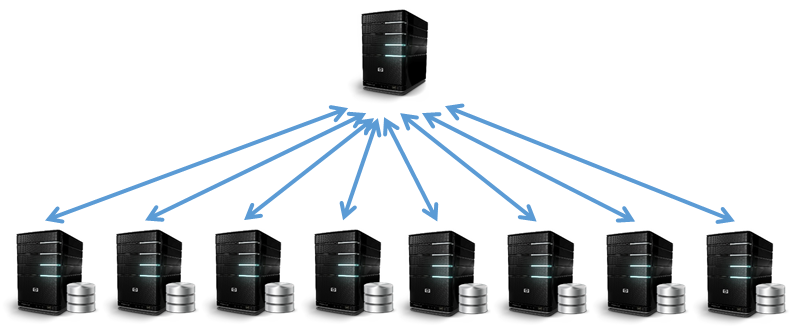
\includegraphics[width=\linewidth]{./mpp_database.png}
        \caption{Banco de dados paralelo e a arquitetura sem compartilhamento.}
        \label{fig:mpp_arq}
\end{figure}

